% Please use the skeleton file you have received in the
% invitation-to-submit email, where your data are already
% filled in. Otherwise please make sure you insert your
% data according to the instructions in PoSauthmanual.pdf
\documentclass{PoS}

\usepackage{siunitx}
\usepackage{subcaption}

\newcommand{\micron}{\si{\micro\meter}}

\title{Pixel Telescope to test pixel Phase II ROCs and sensors}

\ShortTitle{Telescope to Test CMS Upgrade Pixel Detectors}

\author{\speaker{Caleb Fangmeier}\thanks{A footnote may follow.}\\
  Univ.\ of Nebraska \-- Lincoln\\
  E-mail: \email{cfangmei@cern.ch}}

%\author{Another Author\\
%        Affiliation\\
%        E-mail: \email{...}}

\abstract{}

\FullConference{38th International Conference on High Energy Physics\\
		3-10 August 2016\\
		Chicago, USA}


\begin{document}

\section{Introduction}

The innermost layer of the CMS Detector at the LHC is the silicon pixel
tracker. The current version of the detector has performed well and been
critical to the physics program of CMS\@.  The HL-LHC Upgrade of CMS will
replace the entire silicon tracking system.  As part of this upgrade, a
proposed new section of the pixel tracker will be added in the so-called
``very-forward'' ($\eta\sim4$) region of the detector. Because the particles in
this region are traveling almost parallel to the magnetic field of the
detector, enhanced $\phi$ sensitivity is required to accurately measure track
curvature, a critical measurement for finding particle momentum and charge.
Therefore, the proposed detector will reshape the standard
$100\times150\micron$ pixels to be more sensitive in $\phi$, sacrificing
precision in $\rho$. A telescope is being developed for the express purpose of
characterizing different pixel geometries.  The telescope operates by using
eight layers of silicon-strip sensors, with the device-under-test placed with
four on each side. A beam of mimumum-ionizing charged particles is directed so
it passes through both the strip sensors and the the prototype pixel sensors.
Measurements from the telescope are taken to reconstruct individual particle
tracks. These tracks are then compared to data collected from the pixel sensor
to characterize its performance.

\section{Projected Performance}
The performance of the telescope can be quantified in two ways. First, the
precision with which individual particle trajectories can be measured, and
second, the rate at which data can be collected. 

The measurment precision of particle tracks depends on the number of detector
layers and the single hit precision. The telescope consists of eight
silicon-strip-sensor layers with strip-widths of $25\micron$. For strip-sensors
with charge sharing the single hit precision can be approximated by the
strip-width divided by the signal-to-noise ratio (SNR) of the readout system.
The expected SNR of the telescope is 25. This yields a single-hit precision of
$\approx1\micron$. This single-hit precision combined with two measurements in
each dimension on each side of the prototype sensor should give sub-micron
track localization at the point of impact with the prototype sensor.

The data collection rate for the telescope is primarily limited by the speed
sample data can be transferred from the readout chips to the data acquisition
(DAQ) board. This is because many typical test-beam facilities have beam rates
on the order of \si{\mega\hertz} while the telescope can only be triggered at
$\approx15\si{\kilo\hertz}$. The trigger rate can be improved somewhat by
optimizing the readout electronics using well established techniques such as
the placement of buffer amplifiers near the readout chips to reduce the RC time
constant of the cables running from the readout chips to the DAQ board, as well
as making use of differential signaling on these same cables to reduce
electro-magnetic interference. It is because of this limitation that the
decision was made to readout every readout chip in parallel, in contrast with
previous incarnations of this telescope which serialized sixteen readout chips.

\section{Technical Description}
What follows is a a description of the hardware of the telescope and a
high-level overview of the readout scheme.
\subsection{Hardware}
The telescope has been built up around the choice of sensor and accompaning
readout chip, both of which were originally developed for the H1 vertex
detector at HERA\cite{Hilgers2001}. The strip sensor contains 512 strips with
$25\micron$ strip-width. The readout chip is the Analog Pipeline Chip \-- 128
(APC). Each APC can read 128 strips so four are required to read a single strip
sensor. The APC operates an integrating pre-amplifier that collects charge from
the a sensor strip and keeps a 32 sample history of the output of that
pre-amplifier. When a trigger is received from, for example, a scintillation
detector, the appropriate sample is chosen from the 32 based on the calibrated
trigger latency and the samples from all 128 channels of the APC are serialized
to its output.

\begin{figure}[h]
  \centering
  \begin{subfigure}[t]{0.45\textwidth}
    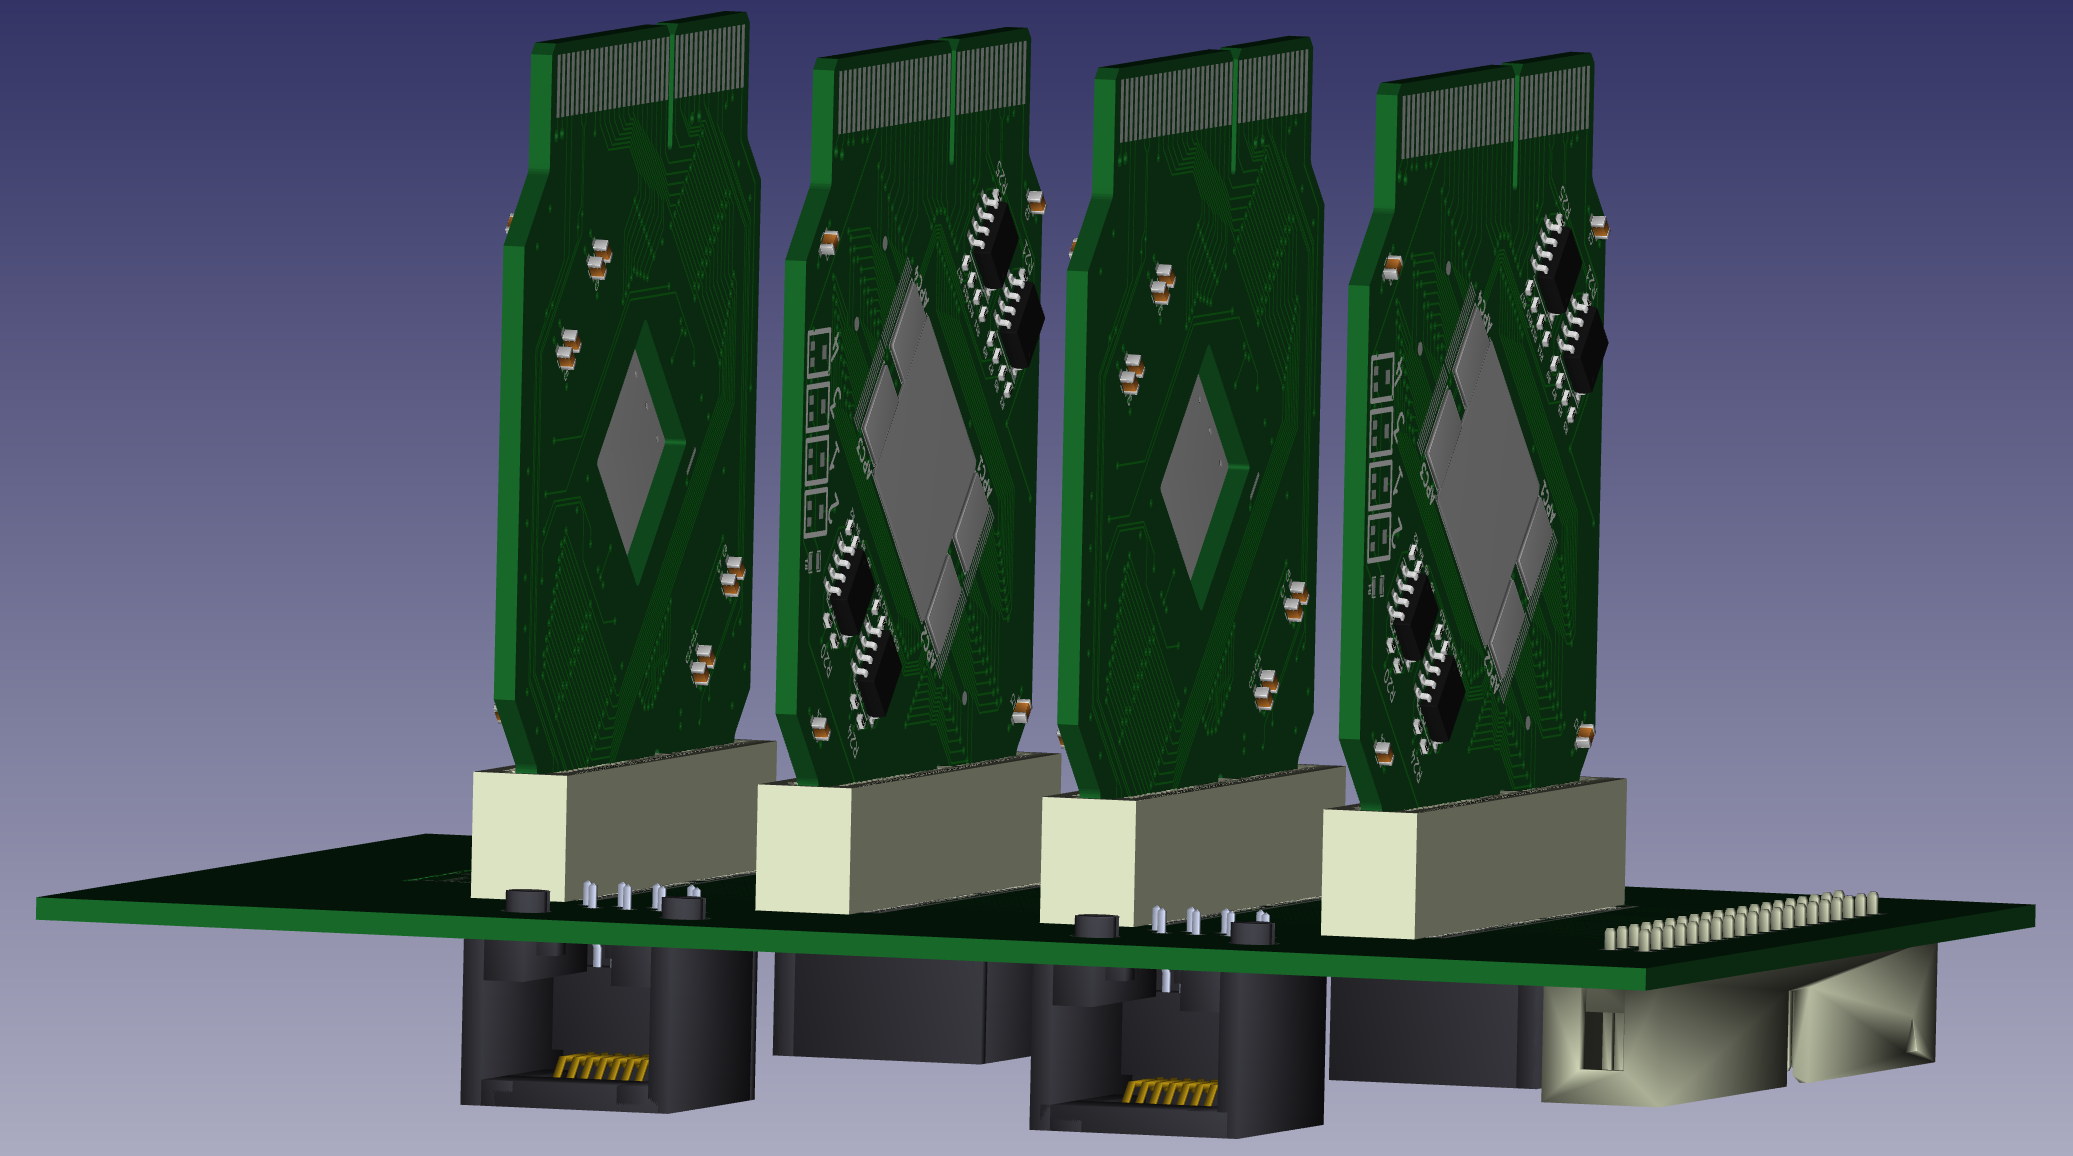
\includegraphics[width=\textwidth]{../figures/Half-Telescope-Full.png}
    \caption{\scriptsize A rendering of the telescope ``motherboard'' showing four
      ``sensor-cards'' each of which holds a single strip-sensor. The control
      signals needed by the readout chip are supplied by a 40-pin header
      (bottom-right). The data readout happens over four RJ-45 connectors, into
      which CAT-5 cables are plugged to transmit the signals to the DAQ board.}
  \end{subfigure}
  \hspace{.3in}
  \begin{subfigure}[t]{0.45\textwidth}
    \includegraphics[width=\textwidth]{../figures/DAQ_Board_Real.png}
    \caption{\scriptsize An image of the data acquisition (DAQ) board featuring an 8xRJ-45
      connector (back) to receive data from two connected motherboards, a
      $2\times40$-pin header (front) for supplying control signals to the
      motherboards, and an Opal-Kelly FPGA integration module (center) to
      orchestrate the operation of the telescope.}
  \end{subfigure}
  \caption{The main hardware components of the telescope are the motherboard with associated sensor-cards (a) and the data acquisition board (b)}
\end{figure}

The strip-sensor along with four APC are mounted onto a ``sensor-card'' along
with four buffer amplifiers that compensate for the relativily weak output of
the APC and generate a more robust differential signal with the proper output
impedance for driving CAT-5 cables ($100\si{\ohm}$). Four sensor-cards are
plugged into a motherboard which provides structural support for the
sensor-cards and routes electrical signals between the sensor cards and the I/O
ports.

\subsection{Readout Scheme}
The readout scheme has been designed to maximize the data throughput in terms
of analog strip-sample values per second. This has been done in an effort to
minimize downtime since the APC cannot take data during readout so any data
from beam that passes through the telescope during readout is lost. Figure 2
illustrates the readout scheme. Roughly speaking, the readout happens in three
stages. The first stage is handled by the electronics in and in the immediate
vicinity of the beam. It is there that the passage of a charged particle is
converted to an electronic pulse by the strip-sensor and the height of that
pulse is recorded by the APC.\ The APC then serializes pulse heights from many
channels to the cables exiting the beam region.

The signals from the 
\begin{figure}[h]
  \centering
  \begin{subfigure}[b]{0.49\textwidth}
    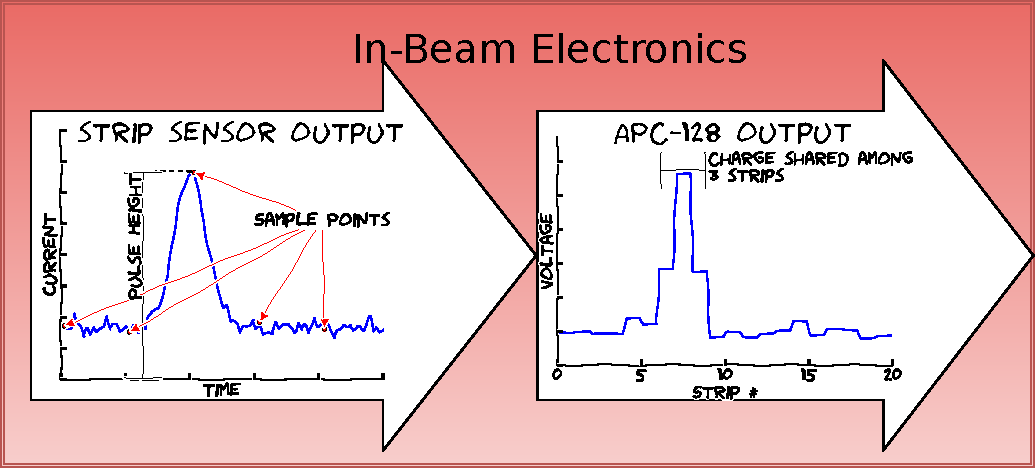
\includegraphics[height=1.32in]{../figures/Telescope_Data_Flow_Stage_I.pdf}
  \end{subfigure}
  \begin{subfigure}[b]{0.49\textwidth}
    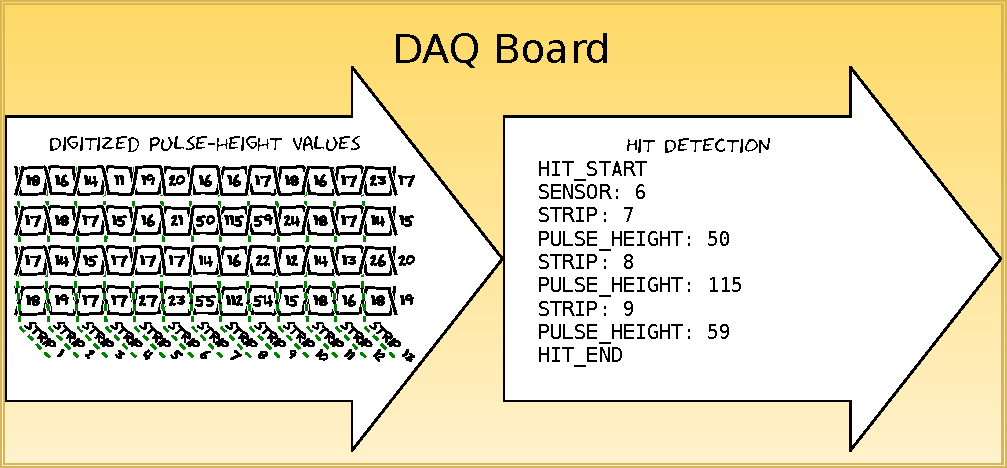
\includegraphics[height=1.32in]{../figures/Telescope_Data_Flow_Stage_II.pdf}
  \end{subfigure}
  \begin{subfigure}[b]{0.49\textwidth}
    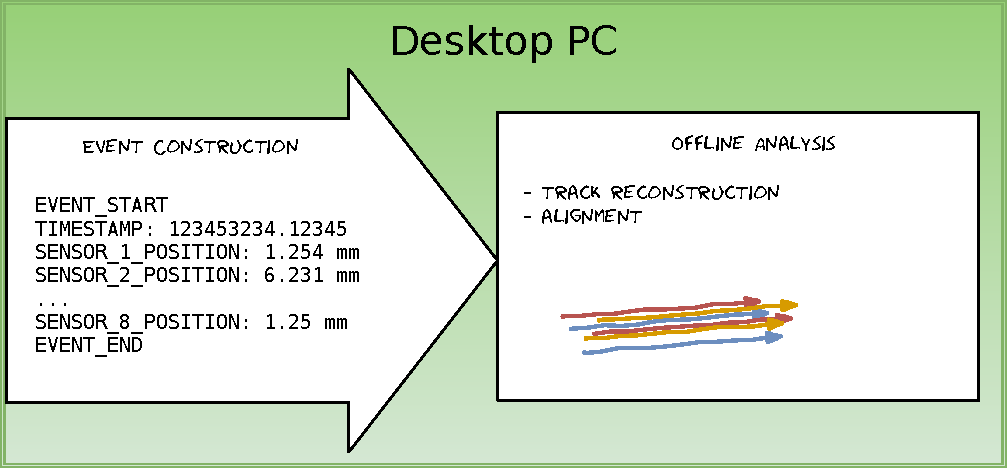
\includegraphics[height=1.32in]{../figures/Telescope_Data_Flow_Stage_III.pdf}
  \end{subfigure}
  \caption{Illustration of the readout scheme of the telescope.}
\end{figure}


\begin{thebibliography}{99}
\bibitem{...}
....

\end{thebibliography}

\end{document}
